\lab{Applications}{Plotting With Matplotlib}{Plotting}
\objective{Introduce some of the basic plotting functions available in Matplotlib}
\label{lab:Matplotlib}

Matplotlib is one of the libraries available for plotting in python.
It is especially good for 2D plotting, but 3D plotting is also possible.

Matplotlib has many different plotting functions.
Table \ref{mpl:basics} is a brief summary of some of the basic 2D plotting functions included in Matplotlib.
We strongly encourage you to visit \url{http://matplotlib.sourceforge.net/} for more information when creating plots.
\begin{table}[h!]
\begin{center}
	\begin{tabular}{|l|p{7cm}|p{3cm}|}

    \hline

    Function & Description & Usage\\

    \hline

    \li{bar} & makes a bar graph & bar(left,height)\\

    \li{barh} & makes a horizontal bar graph & barh(bottom,width)\\

    \li{fill} & plots lines with shading under the curve & fill(x,y)\\

    \li{fill\_between} & plots lines with shading between two given y values & fill\_ between(x,y1, y2=0)\\

    \li{hist} & plots a histogram from data & hist(data)\\

    \li{pie} & make a pie chart & pie(x)\\

    \li{plot} & plots lines and data on standard axes & plot(x,y)\\

    \li{polar} & plots lines and data on polar axes & polar(theta,r)\\

    \li{loglog} & plots lines and data on logarithmic x and y axes & loglog(x,y)\\

    \li{scatter} & plots data, has more options for scatter plots than the plot function & scatter(x,y)\\

    \li{semilogx} & plots lines and data with a log scaled x axis & semilogx(x,y)\\

    \li{semilogy} & plots lines and data with a log scaled y axis & semilogy(x,y)\\

    \li{specgram} & make a spectogram from data & specgram(x)\\

    \li{spy} & plot the sparsity pattern of a 2D array & spy(Z)\\

    \li{triplot} & plot triangulation between given points & triplot(x,y)\\

    \hline

    \end{tabular}
\end{center}
\caption{Some basic functions in Matplotlib.}
\label{mpl:basics}
\end{table}

The basic line plotting function is ``plot". It's default setting plots a set of data points and forms a line between the points. To plot a function we need to input the x and y coordinates of the points we want it to use when plotting. We do this by giving the plot function a list of x values and y values. The coordinates for the points come from corresponding entries in the list. The plot range is taken directly from the data unless we manually set it later.

We can generate a basic plot of $e^x$ using the following lines of code:

\begin{lstlisting}
import numpy as np
from matplotlib import pyplot as plt
x = np.linspace(-2, 3, 501)  # sample x values
y = np.exp(x)  # use sample x values to generate sample y values
plt.plot(x, y)  # call the plot function
plt.show()  # After making a plot we must run the show function to display the output.
\end{lstlisting}

This should display a plot similar to the one shown in Figure \ref{mpl:expplot}.

\begin{figure}
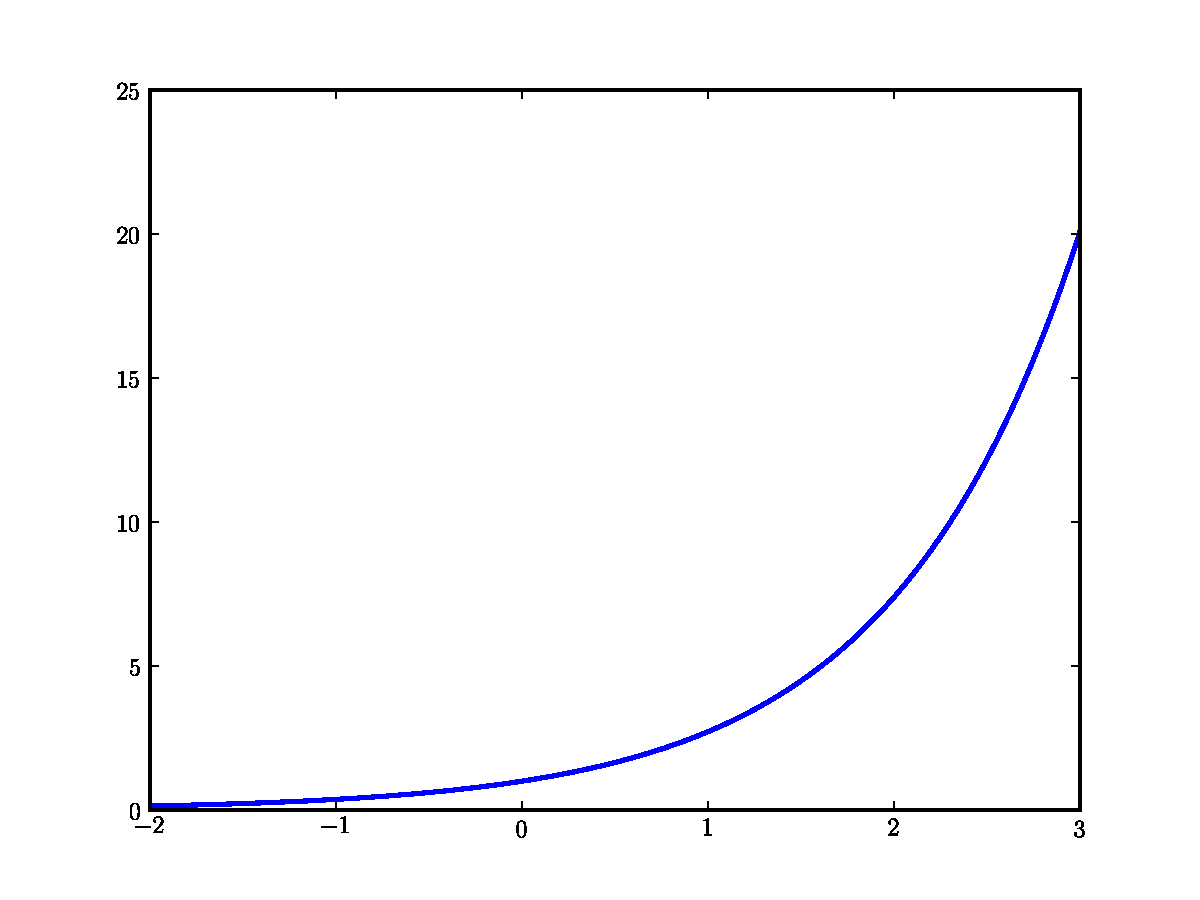
\includegraphics[width=\textwidth]{expplot.pdf}
\caption{A simple plot of $e^x$.}
\label{mpl:expplot}
\end{figure}

Matplotlib plots are pieced together using what is called a state machine environment. What this means is that we can run several different functions and they will all display or modify the plot we are creating. The effects of each function will all be applied to the plot we are making until we either display the plot using the show() function or we clear it.

Pyplot is not the only library built into matplotlib. There are many other features that give us greater freedom with how we make our plots, but we will not cover them here. For more information see:

\url{http://matplotlib.sourceforge.net/users/artists.html}

We can use this state based interface to change many of the plotting options and to join different plots together, for example, the following code can be used to plot lines with random values at integers from 1 to 10.

\begin{lstlisting}
import numpy as np
from matplotlib import pyplot as plt
x = np.linspace(1, 10, 10)
y = np.random.rand(10, 10)
plt.plot(x, y[0], x, y[1], x, y[2], x, y[3], x, y[4], x, y[5], x, y[6], x, y[7], x, y[8], x, y[9])  # the plot function allows for multiple sets of x and y data
plt.show()
\end{lstlisting}

In this example we have used the plot function to plot several different lines at once. We can also overlay different plots onto one another. Using the same x and y that we generated above, the following will give us the same plot:

\begin{lstlisting}
plt.plot(x, y[0])
plt.plot(x, y[1])
plt.plot(x, y[2])
plt.plot(x, y[3])
plt.plot(x, y[4])
plt.plot(x, y[5])
plt.plot(x, y[6])
plt.plot(x, y[7])
plt.plot(x, y[8])
plt.plot(x, y[9])
plt.show()
\end{lstlisting}
Or even a better way to do it is using a loop
\begin{lstlisting}
for n in y:
    plt.plot(x, n)
plt.show()
\end{lstlisting}

A plot that was generated by this code will be similar to the one shown in Figure \ref{mpl:statemachineexample}.

\begin{figure}
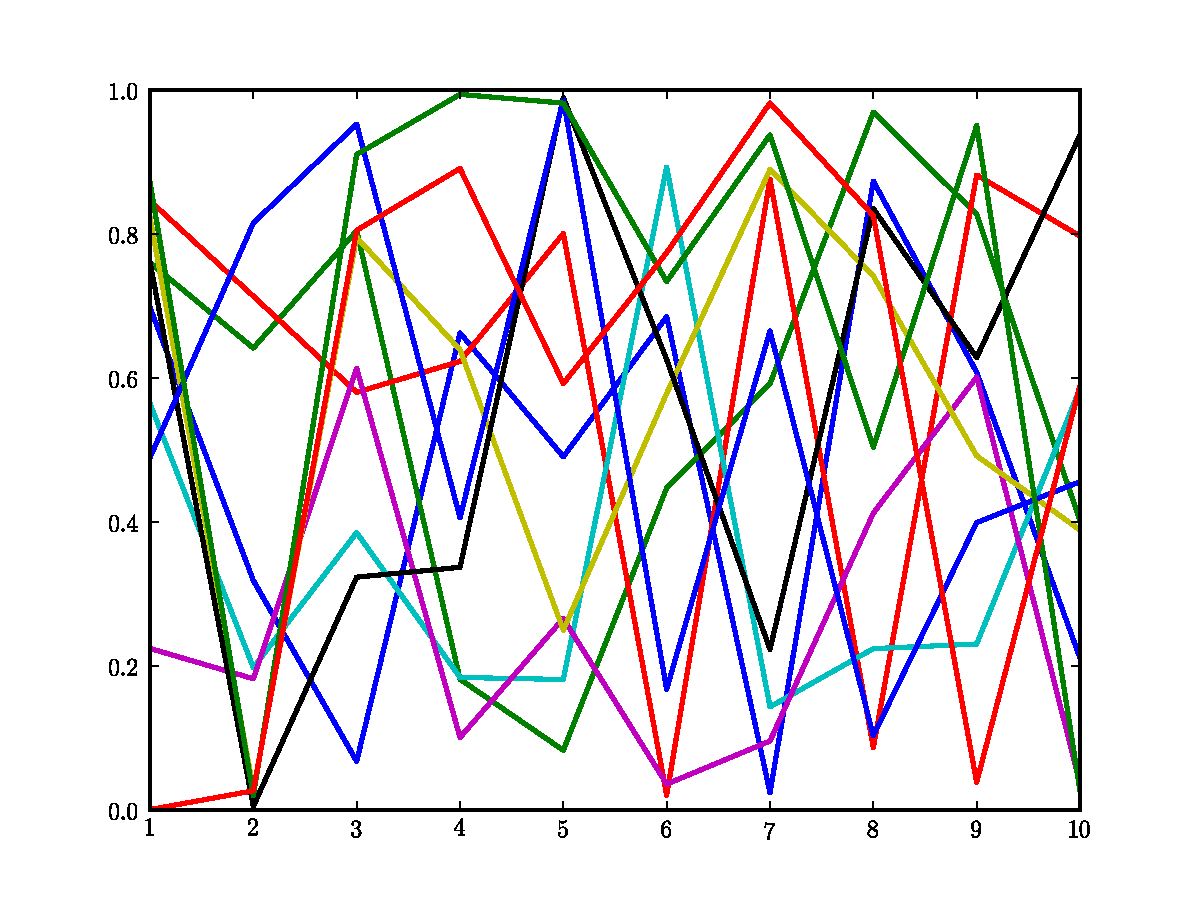
\includegraphics[width=\textwidth]{statemachine.pdf}
\caption{A plot of $10$ lines with randomly generated $y$ values.}
\label{mpl:statemachineexample}
\end{figure}

The lines that we plot in this way do not necessarily have to have the same domain or range.
A suitable domain and range for the plot is chosen automatically unless we specify otherwise.

\begin{problem}
Go to the documentation on the matplotlib website.
Look at the documentation for the plot function.
Plot the function $\sin(x)$ from $0$ to $2\pi$ with a red dashed line and the function $\cos(x)$ on the same domain with a blue dotted line using a single call to the plot function.
\end{problem}

There are also many functions that we may use to set different values in the plotting environment.
A few examples are shown in Table \ref{mpl:useful_functions}.

\begin{table}[h!]
\begin{center}
	\begin{tabular}{|l|p{6cm}|p{4cm}|}

    \hline

    Function & Description & Usage\\

    \hline

    \li{annotate} & adds a commentary at a given point on the plot & annotate('text',(x,y))\\

    \li{arrow} & draws an arrow from a given point on the plot & arrow(x,y,dx,dy)\\

    \li{axhline} & draws a horizontal line at y from xmin to xmax & axhline(y=0, xmin=0, xmax=1)\\

    \li{axvline} & draws a vertical line at x from ymin to ymax & axvline(x=0, ymin=0, ymax=1)\\

    \li{axhspan} & draws a rectangle from xmin to xmax and ymin to ymax, if no xmin and xmax are given it goes across the plot & axhspan(ymin, ymax, xmin=0, xmax=1)\\

    \li{axvspan} & draws a rectangle from ymin to ymax and xmin to xmax, if no ymin and ymax are given it goes across the entire plot & axvspan(xmin, xmax, ymin=0, ymin=1)\\

    \li{figlegend} & place a legend in the plot & figlegend(handles, labels, loc)\\

    \li{grid} & add gridlines & grid()\\

    \li{text} & add text at a given position on the plot & text(x,y,'text')\\

    \li{title} & add a title to the plot & title('text')\\

    \li{xlim} & set the x limits, returns current limits if no arguments are given & xlim(xmin,xmax)\\

    \li{ylim} & set the y limits, returns current limits if no arguments are given & ylim(ymin,ymax)\\

    \li{xticks} & set the location of the tick marks on the x axis, returns current locations if no arguments are given & xticks(x)\\

    \li{yticks} & set the location of the tick marks on the y axis, returns current locations if no arguments are given & yticks(y)\\

    \li{xlabel} & add a label to the x axis & xlabel('text')\\

    \li{ylabel} & add a label to the y axis & ylabel('text')\\

    \hline

    \end{tabular}
\end{center}
\caption{Some Functions to Set Plotting Options}
\label{mpl:useful_functions}
\end{table}

\begin{problem}
Plot the curve $\frac{1}{x-1}$ from $-2$ to $6$.
Force the plot to only show $y$ values that are between $-6$ and $6$.  By default \texttt{plot} will try to make the graph connected.  Correct this so that the graph is discontinuous at $x=1$, as it should be.
\end{problem}

\begin{problem}
Plot the curve $\sin(x)\frac{1}{x+1}$ from $0$ to $10$.
Use blue shading under the curve when it is positive and red when it is negative (Hint: you may want to use the \verb!fill_between! command).
Make the line dotted.
Label the x-axis ``x-axis", the y-axis ``y-axis", and the plot ``My Plot".
Enable the gridlines.

Also include a scatter plot of half of the value of the function at each of it's maxima and minima in the range.
Have it display the points as blue triangles.
Make sure the x limits of the plot are still 0 and 10.
\end{problem}

Some other useful functions available in pyplot include imread, which imports an image as an array, and imshow, which displays an image from an array.

There are also functions in pyplot available to represent 3D plots as contour plots, pseudocolor plots, etc.
The following is an example of using the pcolor function to represent the surface $z=\sin(x)\sin(y)$:
\begin{lstlisting}
import numpy as np
from matplotlib import pyplot as plt
n = 401
x = np.linspace(-6, 6, n)
y = np.linspace(-6, 6, n)
X, Y = np.meshgrid(x, y)
C = np.sin(X) * np.sin(Y)
plt.pcolor(X, Y, C)
plt.show()
\end{lstlisting}
This plot is shown in \ref{mpl:pcolor}

\begin{figure}
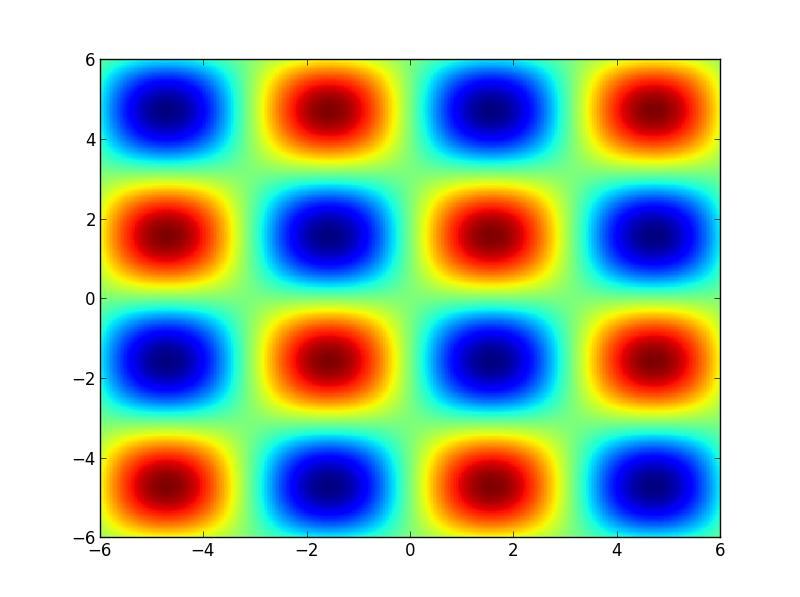
\includegraphics[width=\textwidth]{pcolor.png}
\caption{Color plot of $\sin\left(x\right)\times\sin\left(y\right)$.}
\label{mpl:pcolor}
\end{figure}

\begin{problem}
Pcolormesh is a function similar to pcolor. It is usually faster but not always as robust.
Use plt.pcolormesh to plot the absolute value of the function $x^3 +2x^2 -x +3$ on the complex plane.
The output should look like Figure \ref{mpl:pcolormesh}
\end{problem}

\begin{figure}
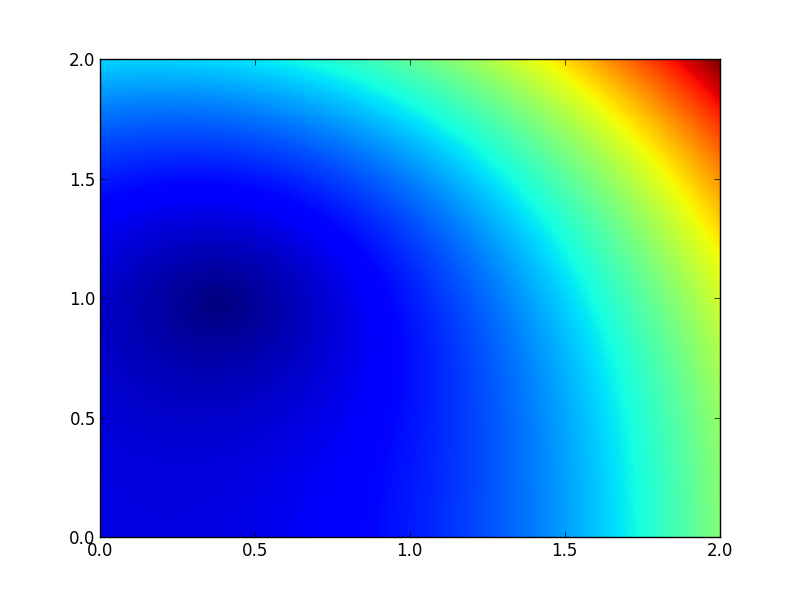
\includegraphics[width=\textwidth]{pcolor2.png}
\caption{Another example of a colorplot.}
\label{mpl:pcolormesh}
\end{figure}

Matplotlib can also be used for 3D plotting.
The following is an example of how to use matplotlib to plot the function $z=\sin(x)\sin(y)$ with both x and y ranging from -6 to 6.
The resulting plot is shown in Figure \ref{mpl:3dplot}.
If you change the number of sample points used you will notice that graphs look much nicer with large numbers of sample points, but it will also take much longer for your computer to render the image.

\begin{lstlisting}
from mpl_toolkits.mplot3d import Axes3D
from matplotlib import pyplot as plt
import numpy as np
fig = plt.figure()
ax = fig.gca(projection='3d')
x = np.linspace(-6, 6, 301)
y = np.linspace(-6, 6, 301)
X, Y = np.meshgrid(x, y)
Z = np.sin(X) * np.sin(Y)
ax.plot_surface(X, Y, Z)
plt.show()
\end{lstlisting}

\begin{figure}
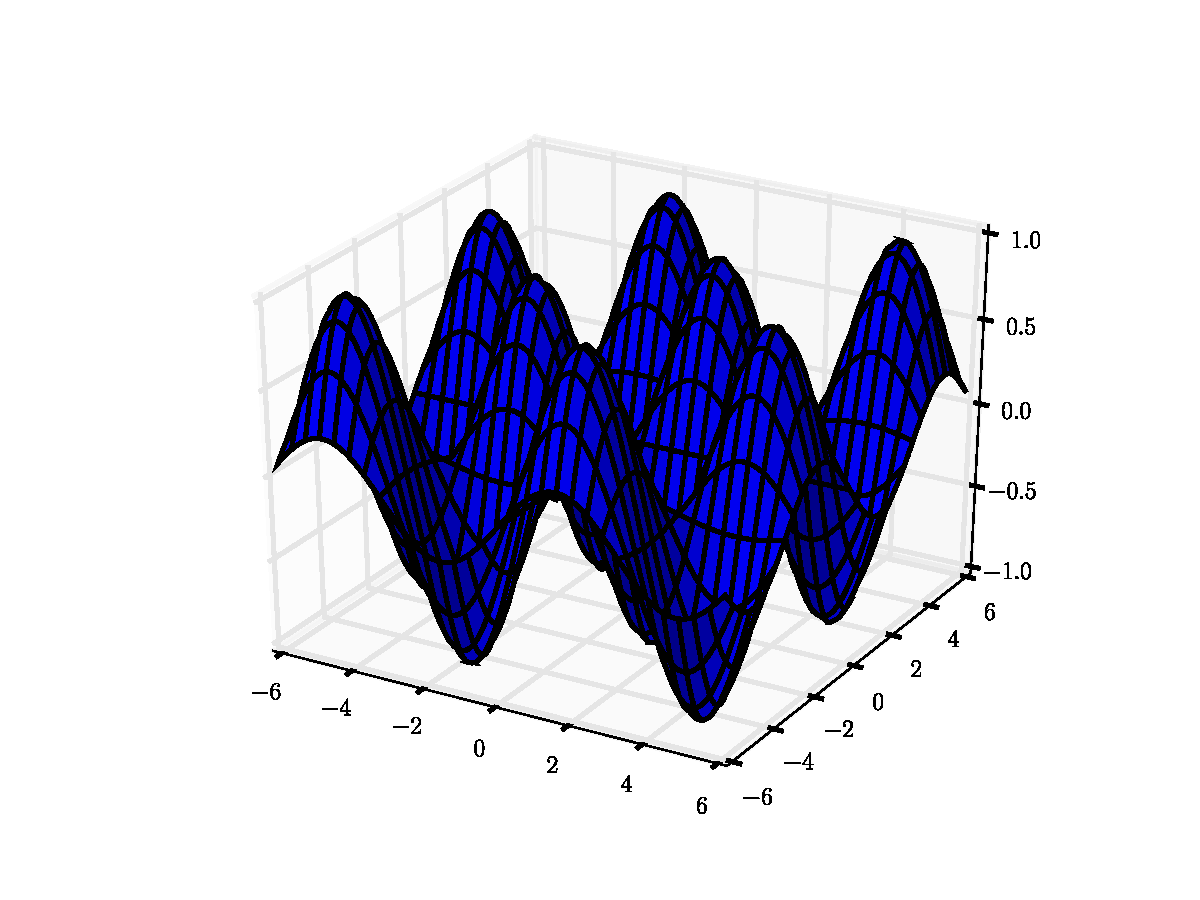
\includegraphics[width=\textwidth]{3dplot.pdf}
\caption{A 3D plot of $\sin\left(x\right)\times\sin\left(y\right)$.}
\label{mpl:3dplot}
\end{figure}

\begin{problem}
Plot the function
\begin{equation*}
\frac{\cos\left(\sqrt{x^2 + y^2}\right)}{\frac{x^2 + y^2}{10} + 1}
\end{equation*}
on $[-10, 10] \times [-10, 10]$.
\end{problem}

Matplotlib also allows us to make interactive graphs as follows:

% This example is largely based on one of the examples in the matplotlib docs.
% I have simplified it and changed the way the libraries are imported, but we could do a citation anyway.

\begin{lstlisting}
import numpy as np
from matplotlib import pyplot as plt
from matplotlib import widgets as wg
ax = plt.subplot(111)
plt.subplots_adjust(bottom=.25)
t = np.arange(0., 1., .001)
a0 = 5.
f0 = 3.
s = a0 * np.sin(2 * np.pi * f0 * t)
l = plt.plot(t, s)[0]
plt.axis([0, 1, -10, 10])
axfreq = plt.axes([.25, .05, .65, .03])
axamp  = plt.axes([.25, .1, .65, .03])
sfreq = wg.Slider(axfreq, 'Freq', .1, 30., valinit=f0)
samp = wg.Slider(axamp, 'Amp', .1, 10., valinit=a0)
def update(val):
    amp = samp.val
    freq = sfreq.val
    l.set_ydata(amp * np.sin(2 * np.pi * freq * t))
    plt.draw()
sfreq.on_changed(update)
samp.on_changed(update)
plt.show()
\end{lstlisting}
The resulting plot is shown in Figure \ref{mpl:interact}.

\begin{figure}
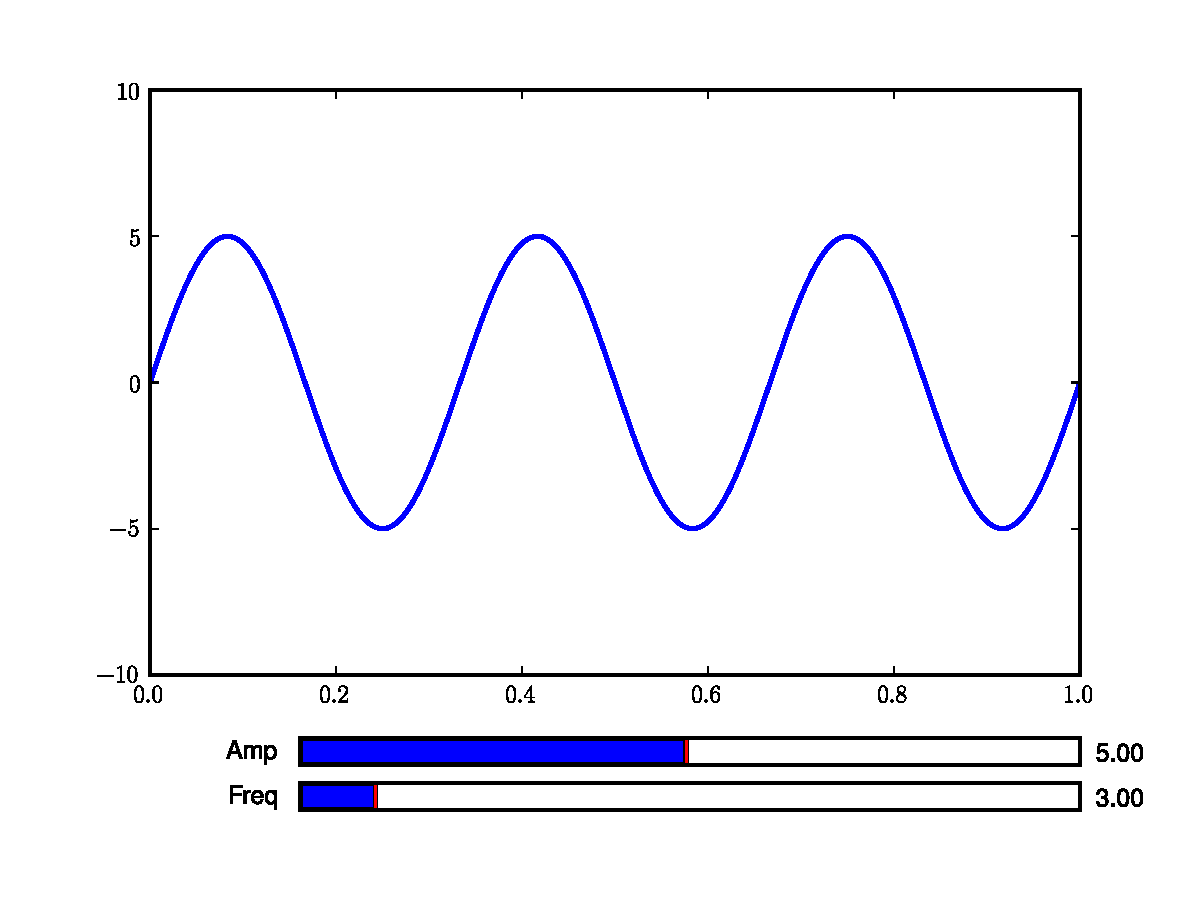
\includegraphics[width=\textwidth]{interact.pdf}
\caption{A snapshot of an interactive plot made using Matplotlib.}
\label{mpl:interact}
\end{figure}

\begin{problem}
Modify the code above to add a third slider to manipulate the phase of the wave shown.
Have it range from 0 to $2\pi$ and set the default value to zero.
\end{problem}

We can also use the plt.subplot command to plot multiple images at the same time.
We can control the different options for each of the subplots in the same way we would for the entire plot.
We change each subplot by using the subplot to set which subplot we are working on, and then writing the code to plot it from there.
In the following example we show plots of $sin x$ and $cos x$ on two different axes within the same plot.
Figure \ref{mpl:subplots} is the output from the following code:
\begin{lstlisting}
import numpy as np
from matplotlib import pyplot as plt
x = np.linspace(-np.pi, np.pi, 400)
y1 = np.sin(x)
y2 = np.cos(x)
plt.subplot(211)
plt.plot(x, y1)
plt.subplot(212)
plt.plot(x, y2)
plt.show()
\end{lstlisting}

\begin{figure}
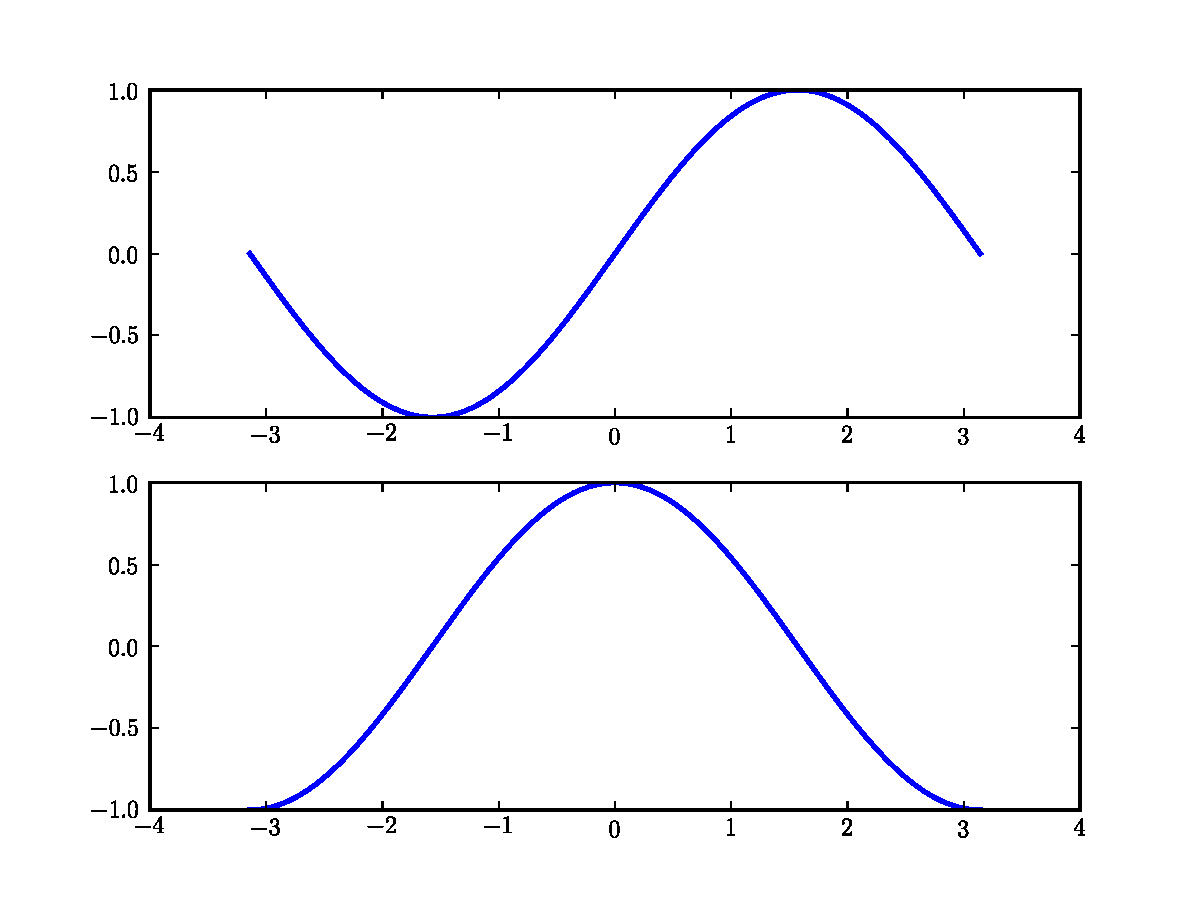
\includegraphics[width=\textwidth]{subplots.pdf}
\caption{An example of the use of subplots in Matplotlib.}
\label{mpl:subplots}
\end{figure}

The subplot command takes a 3 digit number which indicates how we are dividing up the graph and which subplot we are editing.
The first number indicates how many rows there are.
The second number indicates the number of columns.
The third indicates where the subplot is on the grid that we have set up.

We can add titles to each subplot using the \li{plt.title} function.
The \li{plt.suptitle} function allows us to give the entire figure a title as well.

\begin{problem}
Make a plot with 4 subplots.
In the subplots place graphs of $e^x$, $sin(x)$, $cos(x)$, and $x^2$.
Plot all of them on the interval $(-\pi,\pi)$.
Title each of them accordingly.
Title the entire figure ``My Different Plots."
\end{problem}
